\documentclass[11pt]{article}

% Load packages
\usepackage{amsmath, amsfonts} % for math
\usepackage{graphicx} % for figures
\usepackage[margin=1in]{geometry} % to set margins
\usepackage{tcolorbox} % to create nice boxes
\tcbuselibrary{skins,breakable} % extra libraries for the nice boxes
\usepackage{listings}
\usepackage{enumerate}
\usepackage{empheq}
\usepackage{caption}

% Define a custom box for the solutions. Don't change this!
\newtcolorbox[]{solution}
    {colframe=red!20, 
        colback=white, 
        sharp corners,
        title=Solution,
        enhanced,
        coltitle=black,
        fonttitle=\bfseries,
        attach boxed title to top left={yshift*=-\tcboxedtitleheight/2, xshift=3mm},
        boxed title style={sharp corners, colback=red!20}
        }

\usepackage{boondox-calo}

\newcommand{\lr}[1]{\left(#1\right)}

\usepackage{hyperref}
\hypersetup{
    colorlinks=true,
    linkcolor=blue,
    filecolor=magenta,      
    urlcolor=cyan
}

% MSE Set graphics path
\graphicspath{{figs/}}

% MSE Terminal environment for screenshots
\lstdefinestyle{Terminal}
{
    basicstyle=\fontsize{9}{11}\color{black}\ttfamily
}

% MSE Code snippets
\lstdefinestyle{CodeSnippet}
{
    basicstyle=\fontsize{10}{12}\color{black}\ttfamily
}
% MSE Macros
\newcommand{\tty}[1]{\texttt{#1}}

% Write the document
\begin{document}

    \title{Extreme Computing: Homework 2}
    \author{Michael S. Emanuel, Jonathan Guillotte-Blouin, Yue Sun}
    \date{April 15, 2019}
    \maketitle

  \section{Problem 1:  Channel Flow with a central narrowing}
    Simulating channel flow in 2D with a narrowing is the target.

The type of flow in absence of the narrowing is the well-known Hagen-Poiseuille flow 
(and by the way, Poiseuille was a physicist and physiologist who studied blood flows 
in a systematic way).

Let's write the corresponding grid for a straight channel aligned along, say, the x axis. 

When constructing the grid and using it in the LBM context 
you should apply what you have learned about grid management. 

Let's recall that in absence of open boundaries (inlet or outlet), each fluid node should always 
be surrounded by other fluid or wall nodes to preserve mass and momentum locally (no leakage rule).

The solution should employ two different options:

    \begin{enumerate}
      \item A periodic channel (aligned with the x direction): start from a quiescent fluid and
      apply a body acceleration uniformly through the fluid until you match the Reynolds number at steady state.
      \item A non-periodic channel with inlet and outlet faces and by applying a uniform velocity 
      at inlet and outlet with plug flow profiles.
    \end{enumerate}

    Use no-slip boundary conditions at the walls and a Reynolds number of $10^{-2}$ computed from fluid velocity 
    imposed at $x=0$ (the inlet region for non-period channel) and characterstic length being $H$.

    \begin{figure}[h!]
      \centering{}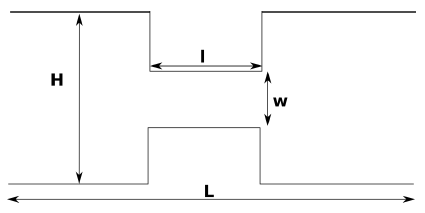
\includegraphics[scale=1.0]{narrowing.png}
      \caption{The geometry for the channel with central narrowing.}
      \label{fig:narrowing}
    \end{figure}

    
    \textbf{For a fixed set of values for the geometry 
    as in Fig. \ref{fig:narrowing}, (suggested values $L=200$, $H=60$, $l=50$, $w=30$), 
    calculate the following quantities:}
    \begin{enumerate}
      \item The pressure field
      \item The velocity field 
      \item The volume flow rate 
      \item The average and maximum velocities in the channel
    \end{enumerate}

    Repeat the simulation by varying the width of the narrowing $w$.

\textbf{Code Overview}

Our solution to this problem can be found in the folder \tty{hw2/lbm\_7}
in our team's repository for this course.  
Here is a brief overview of the components in our solution.

The file \tty{lattice.hh} declares and implments the class \tty{lattice}
(that is, it's a header-only implemenation).  
One instance of this class represents a single point on the lattice.
It keeps track of populaations $p_0$ through $p_8$ and their equilibrium values. 
It also tracks the hydrodynamic values $\rho$, $u_x$, $u_y$ and $p$ (pressure).
The function  \tty{hydro} computes the hydodynamic variables as a function of the populations.
The function \tty{equilibrium} computes the equilibrium populations as a function of the hydrodynamic macro quantities.
The function \tty{collide} does the post-collision update, relaxing each population towards the equilibrium.
The parameter \tty{tau} controls the rate of relaxation to equilibrium.
As we learned in class, there is a linear relationship between $\tau$ and the kinematic viscosity $\nu$, namely
$$\nu = \frac{2\tau-1}{6}$$

The files \tty{lbm.hh} and \tty{lbm.cc} declare and implment the class that builds
the overall Lattice Boltzmann grid.  
This class has member variables tracking the parameter values for the simulation, including
the Reynolds Number \tty{Re}, the relaxation time $\tau$, 
the kinematic viscosity $\nu$, and the length scale \tty{D}.  
The number of grid points in the x and y directions are \tty{nx} and \tty{ny}.
We use the strategy recommended by Sauro Succi and include buffers around the outside.
We chose direct addressing rather than indirect addressing for this problem because the
grid is rectilinear and dense.
The biggest member variable is a pointer to an array of lattice objects, named \tty{f}.
There is also a Boolean array of obstace indicators \tty{obs}.

The initialization routines parallel the lattice class and Sauro's scheme.
Methods include \tty{initialize}, \tty{init\_hydro}, \tty{init\_flow}, 
\tty{init\_poiseuille}, \tty{init\_sstpoiseuille} (sst is for steady-state),
and \tty{init\_pop}.
The solution is methods include the following:
\tty{solve}, \tty{bc}, \tty{pbc}, \tty{mbc}, \tty{stream}, \tty{hydro},
\tty{equilibrium}, \tty{collide}, \tty{force}, \tty{obstacle}, and \tty{set\_channel}.
The post-processing methods include \tty{set\_dir} and \tty{output}.

The driver programs are \tty{lbm\_pbc} and \tty{pbm\_mbc}.  
These handle the periodic boundary condition and mixed boundary with forcing, respectively.
There isn't too much happening in the driver programs; 
the heavy lifting is done in the \tty{lattice} and \tty{lbm} classes.
Each driver sets up the main problem instance, solves it, and writes the output.
They then enter a loop where different widths $w$ are simulated, 
for $w$ in the range $10, 20, 30, 40, 50$.
In the periodic boundary driver \tty{lbm\_pbc} only, 
we also have an additional loop over relaxation times $\tau$ 
in the range 0.65, 0.70, 0.75, 0.80, 0.85, 0.90, 0.95, 1.00.
These correspond to kinematic viscosities in the range 0.05 to 0.1667
and address the last part of question 1.

Finally a good deal of post-processing is done in a Jupyter notebook called \tty{viz.ipynb}.
This started out limited to visualization, but we also compute 
some summary statistics asked for below.  
The common approach is to open a directory of frames containing one simulation run.
Typically we use only the last frame, to answer questions about the end of the 
simulation which should be close to steady state.

The question specifically asks that we compute the pressure field, velocity field,
volume flow rate, and the average and maximum velocities in the channel.
Each frame includes entries at every grid point for:
\begin{itemize}
\item the density $\rho$
\item the x-velocity $u_x$
\item the y-velocity $u_y$
\item the pressure $p$
\end{itemize}

We compute the speed $v$ in post-processing as $v = \sqrt{u_x^2 + y_y^2}$.
We will present our results for the four fields as plots in the base case at
end end of the simulation (frame 99).

%Periodic
% pressure
\begin{center}
\begin{figure}
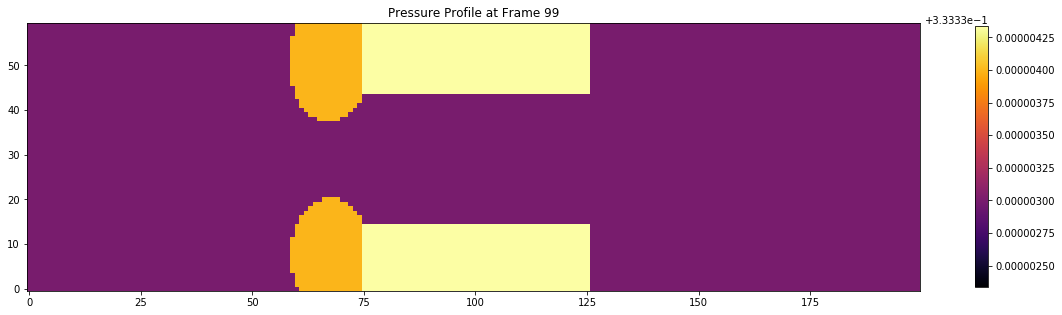
\includegraphics[width=0.90\textwidth]{lbm_pbc_pressure.png}
\captionof*{figure}{Periodic: Pressure Field}
\end{figure}

% ux
\begin{figure}
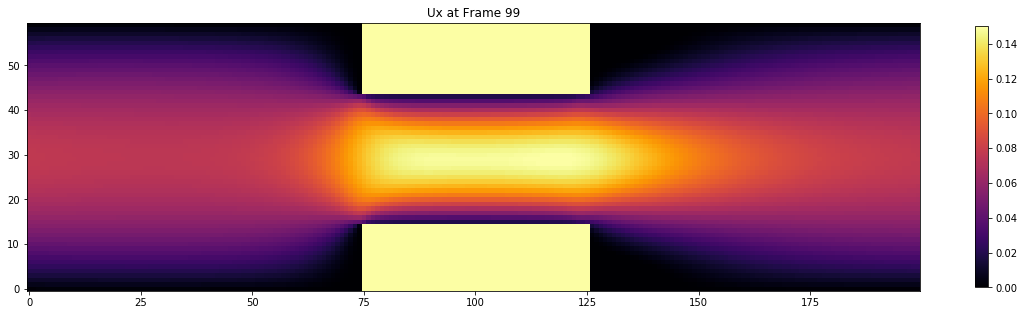
\includegraphics[width=0.90\textwidth]{lbm_pbc_ux.png}
\captionof*{figure}{Periodic: Velocity in x-direction $u_x$}
\end{figure}

% uy
\begin{figure}
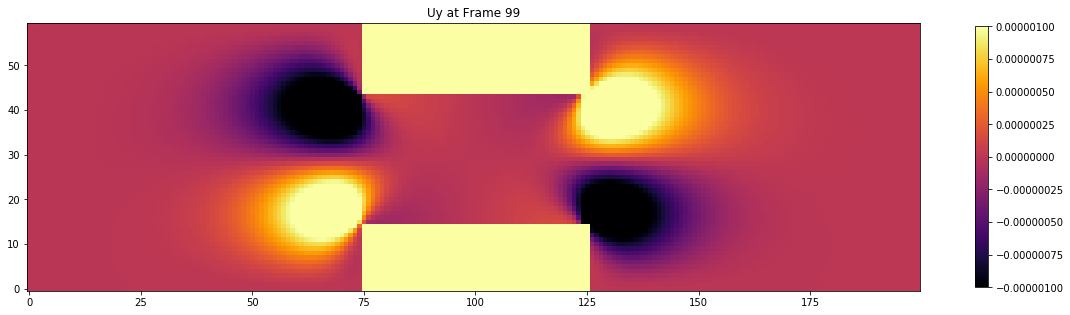
\includegraphics[width=0.90\textwidth]{lbm_pbc_uy.png}
\captionof*{figure}{Periodic: Velocity in y-direction $u_y$}
\end{figure}

% speed
\begin{figure}
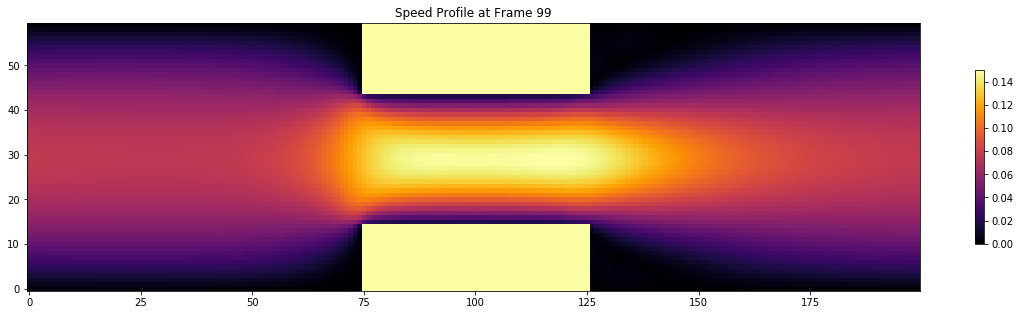
\includegraphics[width=0.90\textwidth]{lbm_pbc_speed.png}
\captionof*{figure}{Periodic: Speed $v$}
\end{figure}
\end{center}

%Non-Periodic
% pressure
\begin{center}
\begin{figure}
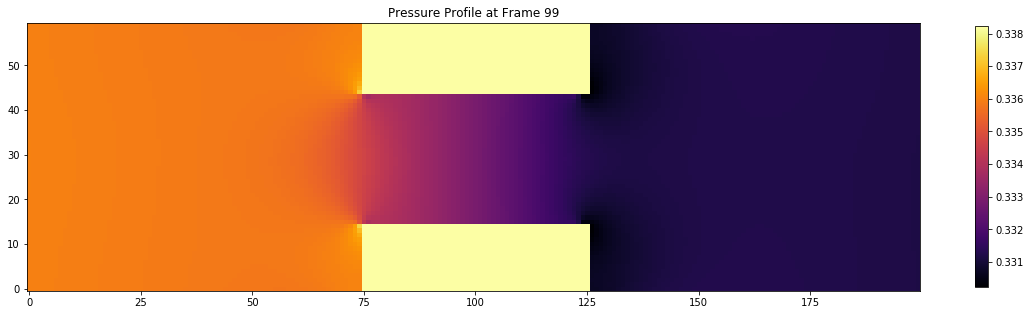
\includegraphics[width=0.90\textwidth]{lbm_mbc_pressure.png}
\captionof*{figure}{Non-Periodic: Pressure Field}
\end{figure}

% ux
\begin{figure}
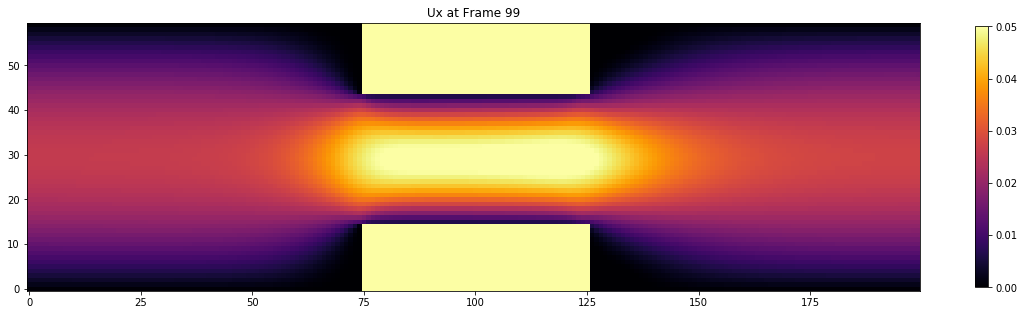
\includegraphics[width=0.90\textwidth]{lbm_mbc_ux.png}
\captionof*{figure}{Non-Periodic: Velocity in x-direction $u_x$}
\end{figure}

% uy
\begin{figure}
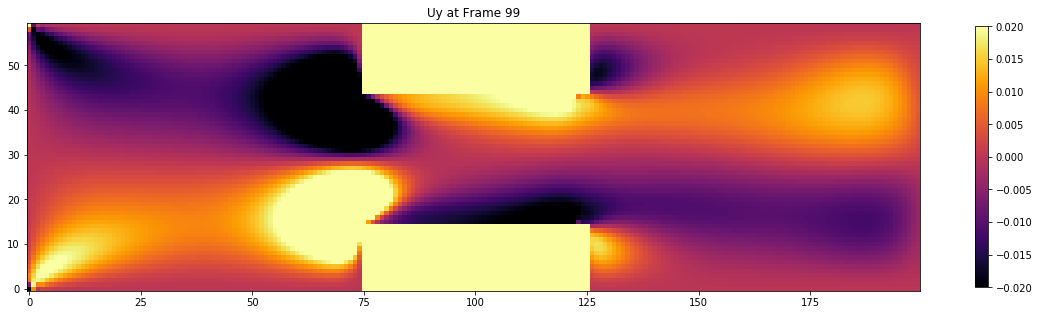
\includegraphics[width=0.90\textwidth]{lbm_mbc_uy.png}
\captionof*{figure}{Non-Periodic: Velocity in y-direction $u_y$}
\end{figure}

% speed
\begin{figure}
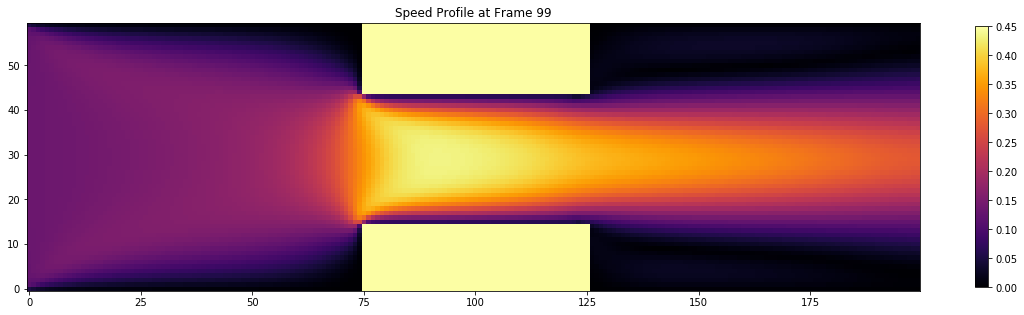
\includegraphics[width=0.90\textwidth]{lbm_mbc_speed.png}
\captionof*{figure}{Non-Periodic: Speed $v$}
\end{figure}
\end{center}

We computed the speed in the channel and the flow rate as a post-processing step in \tty{viz.ipynb}
\begin{itemize}
\item Periodic: mean speed 0.050695, max speed 0.150508, volume flow 3.04553
\item Non-Periodic: mean speed 0.017598, 0.053161, volume flow 1.046670
\end{itemize}

We computed the volume flow rate as the amount of fluid passing a vertical line
at a given value of $x$.  We would expect that this would be equal for any $x$ 
we chose at steady state by conservation of mass.  This is close to being true.
We therefore chose to take the mean of this quantity across all the $x$ values
in our grid to get the most accurate estimate of the volume flow.
As a sanity check, we printed out the volume flow every 20 steps from $x=0$ to 
$x=200$.  The results were all within 0.02 of the mean, except for the point
at x-100 in the middle of the inlet, where it was 0.08 below the mean.

Here are a few comments about these plots.
There is a significant difference in the scale of the speed and volume flow rate between
the periodic and non-periodic cases.
We have double checked our work and believe it to be correct.
The problem statement is in terms of a target Reynolds number, 
and the way we are calibrating the fluid speeds to achieve this is
quite different between the two cases.
We have confidence that each simulation is correct as presented.

The overall pressure profile is encouraging.  
The pressure varies only very slightly, as we expect for an incompressible fluid simulation.
The variations make sense too, as the modeled pressure is slightly higher on
the left and lower on the right.
The profile of the x-velocity $u_x$ is intuitive; the fluid needs to speed up
considerably in the narrowing for the flow to conserve mass.
We can also see it slowing down next to the boundary due to the 
no-slip boundary condition.
The y-velocity pattern shows very little flow in the y direction,
with four small pockets next to the four corners where the fluid
needs to narrow then widen out to pass through the narrow channel.
Overall these results make sense and look good to us.
Finally, we did a comparison of these results aganst the analytical
results for the PBC and found a good agreement.

    \textbf{Plot:}
    Show how the flow rate changes by varying $w$ in the range $0<w<50$

We simulated $w$ values at 10, 20, 30, 40 and 50.
Towards the bottom of \tty{viz.ipynb}, we have a small function that computes
the volume flow rate for a simulation as described above.
We use it to assemble the volume flows for these widths in both the 
periodic and non-periodic boundary conditions.
Here are the requested plots:
\begin{center}

\begin{figure}
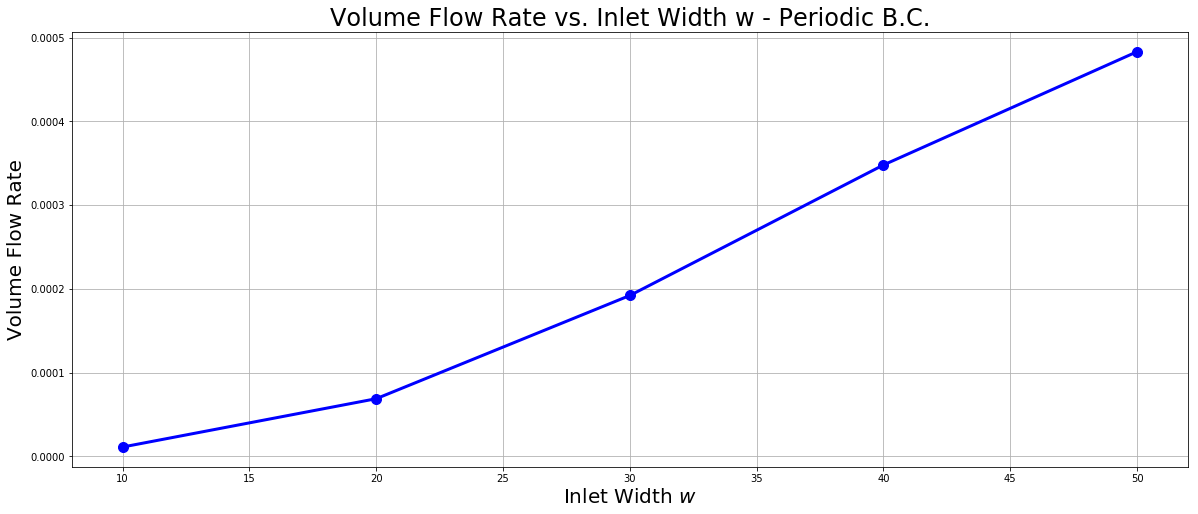
\includegraphics[width=0.90\textwidth]{lbm_pbc_flow_vs_w.png}
\captionof*{figure}{Periodic: Flow vs. Channel Width $w$}
\end{figure}

\begin{figure}
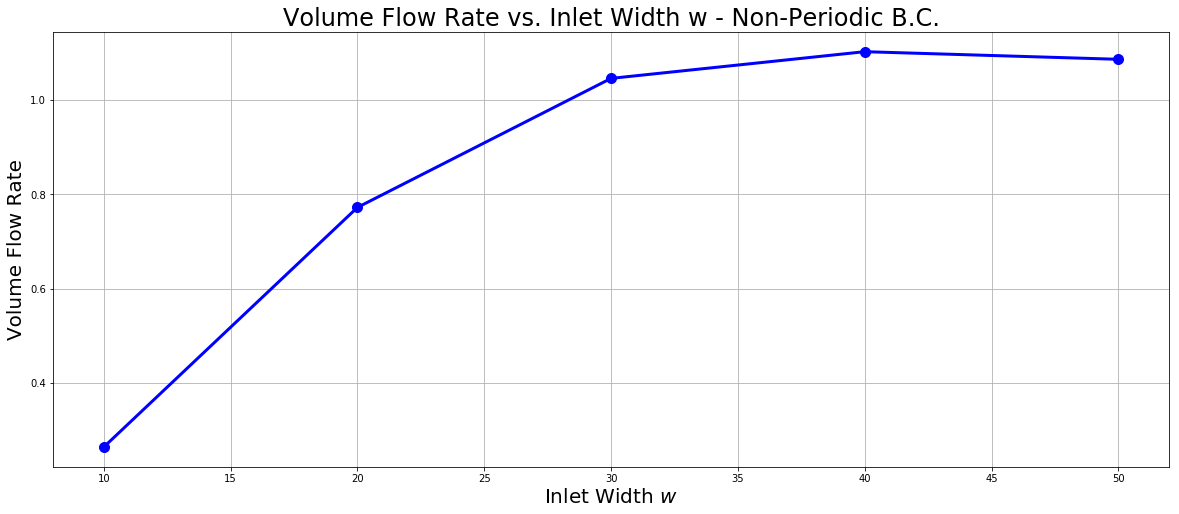
\includegraphics[width=0.90\textwidth]{lbm_mbc_flow_vs_w.png}
\captionof*{figure}{Non-Periodic: Flow vs. Channel Width $w$}
\end{figure}
\end{center}

As expected, we see that the volume flow rate increases for the periodic case with a roughly parabolic shape.  
The flow rate also increases for the non-periodic case, but plateaus past a width of 30.
However, we need to be very careful with our intuition here, because we've standardized on a Reynolds number
 of 0.01 rather than a pressure gradient.  Our intuition about how the flow depends on the width of the 
opening is based on varying the width while holding the pressure gradient constant.
This simulation isn't calibrated that way, so it's measuring something slightly different,
especially in the non-periodic case.

    Compare the pressure at the narrowing with the simple Bernoulli estimate for inviscid flows, stating that
    $$
    \frac{1}{2} \rho u_o^2 + p_o = \frac{1}{2} \rho u_i^2 + p_i
    $$
    where $u_o$ and $p_o$ are cross-sectional averages of velocity and pressure at $x=0$ for a periodic system 
    or at the inlet otherwise, and $u_i$ and $p_i$ are the same quantities at the center of the narrowing. 

We calculate this for the periodic flow case in the next section of \tty{viz.ipynb}.
We begin by computing both sides of the Bernoulli relationship in the base case as a sanity check for the method.
Using the quantities $p_0$, and $u_0$ at $x=0$ (start of the channel) we find an energy density of 0.339.
Using the quantities $p_i$ and $u_i$ at $x=100$ (center of the channel) we find an energy density of 0.334.
Since we expect these to be approximately equal, it's encouraging that they are this close together.
In the Python function \tty{calc\_pressure\_narrow} we calculate the pressure $p_i$ that would be implied
at the narrowest point of the channel by solving this relationship for $p_i$ in terms of $p_0$, $u_0$ and $u_1$.
    \textbf{Plot:}
    Plot the obtained pressure vs the Bernoulli estimate by varying the LBM kinematic viscosity in the range 0.05 : 0.1667.
\begin{center}
\begin{figure}
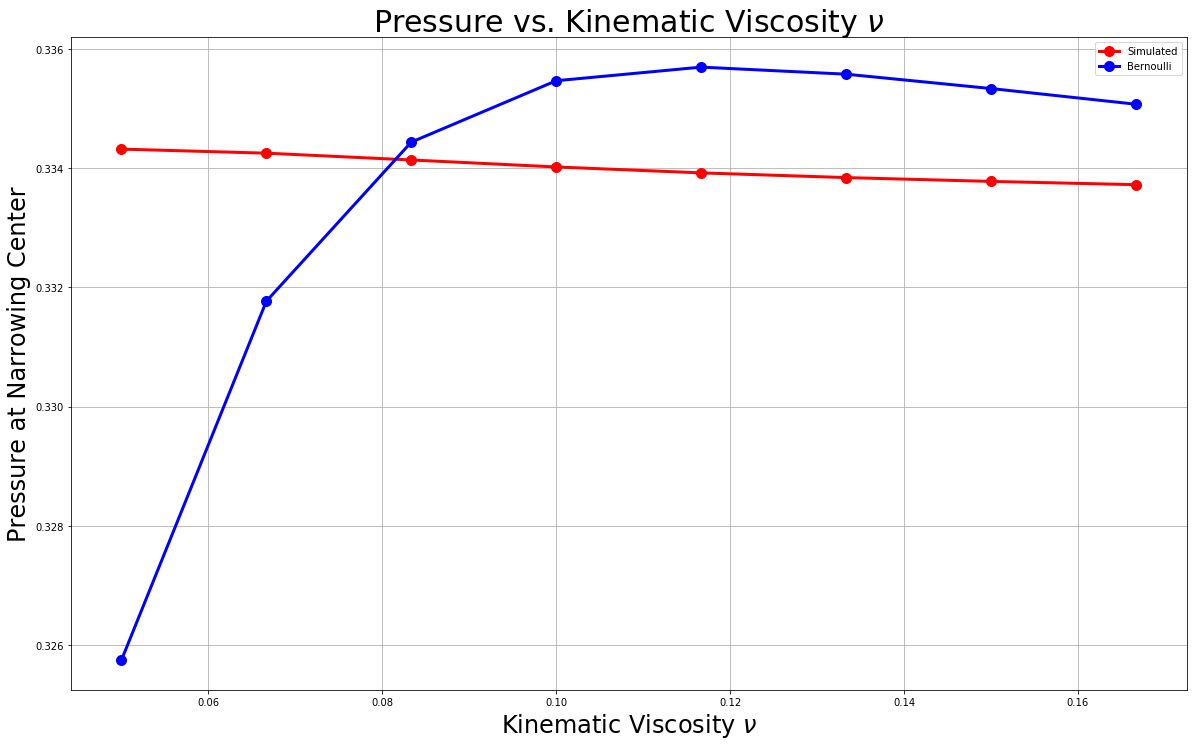
\includegraphics[width=0.90\textwidth]{lbm_pbc_pressure_vs_nu.png}
\captionof*{figure}{Non-Periodic: Flow vs. Channel Width $w$}
\end{figure}
\end{center}  

The scale on this plot is very compressed, so it's important not to overreact to the shape of the curves being different.
The high level story here is the pressure scale ranges from 0.326 to 0.336, so the two methods are actually
in quite good agreement over this range of viscosities.
One thing the chart does seem to be suggesting is that that the Bernoulli approximation is breaking down at an
accelerating rate as the viscosity drops in the range of 0.05.
This isn't too surprising, when we recall that it's an ``inviscid'' approximation.
That approximation will be more accurate at higher viscosities.

%%% PROBLEM 2 %%%
\newpage
  \section{Problem 2:  Basic CUDA and GPUs}
    \textit{This problem was submitted by Dan Willen \texttt{daniel.p.willen@gmail.com}}

    Consider the equation
    \begin{equation}\label{eq:heat}
      \frac{\partial u}{\partial t} = D \nabla^2 u,
    \end{equation}
    on the domain \(0 \leq x,y \leq \pi\), with \(u = u(x,y,t)\), \(D\) the diffusive constant, and \(\nabla^2\) the Laplace operator.
    The boundary conditions are of the homogeneous Dirichlet type:
    \begin{equation}
      u(x = 0, y) = u(x = \pi, y) = u(x, y = 0) = u(x, y = \pi) = 0,
    \end{equation}
    and the initial condition is
    \begin{equation}
      u(x,y, t = 0) = \sin(x) \sin(y).
    \end{equation}
    The solution to this equation is
    \begin{equation}
      u(x,y,t) = \sin(x) \sin(y) \exp{(-2Dt)}
    \end{equation}
    
    Using a second-order central difference in space and first order forward difference in time, the discretization of \eqref{eq:heat} is
    \begin{equation}
      u_{i,j}^{\left(n+1\right)} = u_{i,j}^{\left(n\right)} + \frac{D \Delta t}{\Delta x^2} 
        \left[u_{i+1, j}^{\left(n\right)} +
              u_{i-1, j}^{\left(n\right)} +
              u_{i, j+1}^{\left(n\right)} +
              u_{i, j-1}^{\left(n\right)} -
              4u_{i, j}^{\left(n\right)} \right],
    \end{equation}
    where \(u_{i,j}^{\left(n\right)}\) is the value of \(u\) at the \(n^{th}\) time step at grid point \((i,j)\), \(\Delta t = \Delta x^2 / 4D\) is the time step size, and \(\Delta x\) is the grid spacing in the \(x\) and \(y\) directions.
    
    \vspace{5mm}
    
    \begin{enumerate}
      \item Using Cuda, solve the discretized equations up to a time \(t = \pi^2/D\) using the Jacobi method.
        A skeleton code is provided to assist you, with comments in the locations you should make changes.
        \begin{enumerate}[Step I --]
          \item Declare, allocate, and initialize memory for the field variable \texttt{u} on the CPU.
            You should allocate enough memory for the grid, which has size \(nx \times ny\) and initialize \texttt{u} to the initial condition.
            Make sure you free the memory at the end of the program.
          \item Declare and allocate the GPU memory for \texttt{\_u}, \texttt{\_u\_new}\, and \texttt{\_error}.
            Copy the CPU memory to the GPU; the other two arrays have been initialized to zero for you.
            Make sure you free the memory at the end of the program.
          \item Set up the kernel execution configuration for the GPU kernel based on the input domain size and the maximum threads per dimension,
            which is set at the top of the file as a \texttt{\#define}.
            You will need to determine the number of threads per block and the number of blocks in each direction, as well as set up the \texttt{dim3} variables.
          \item Write a GPU kernel that advances to the next timestep using the Jacobi method.
            This should be done in parallel, not in serial.
          \item Write a GPU kernel that calculates the error between the numerical and analytic solutions at each point.
            Be careful to compare solutions at the correct timestep -- \texttt{\_u\_new} is at \(t = (n+1) \Delta t\) and \texttt{\_u} is at \(t = n \Delta t\).
            Using this result, a parallel reduction using the Thrust parallel algorithms library has been provided to calculate the total error in order to find the average percent error at each grid point.
          \item At the end of the loop, copy the data back to the CPU.
        \end{enumerate}
    \end{enumerate}
    
    Your program should take as an input the number of grid cells on one side of the domain.
    This has been set up for you such that the program can be run from the command line like: 
    \vspace{3mm}\\ \texttt{./jacobi\_solver.cu n} \vspace{3mm}\\
    where \(nx = ny = \) \texttt{n} is the size of one side of the square domain.
    The program should output the percent difference between your result and the analytic solution, averaged over all of the grid nodes:
    \begin{equation}
      \epsilon = \frac{1}{n_x n_y} \sum_{i=1}^{n_x} \sum_{j=1}^{n_y} \frac{u_{i,j}^{\left(n\right)} -
U_{i,j}^{\left(n\right)}}{U_{i,j}^{\left(n\right)}},
    \end{equation}
    where \(U\) is the analytic solution.
    
\textbf{Code Overview}
Our solution to this problem can be found in the folder \tty{hw2/jacobi} in our team's repository for this course.
Here is a brief overview.  There is only one source code file in this solution, \tty{parallel.cu},
plus a short Makefile.  We will say a few words about the six steps described in the algorithm overview.

In step I, we declare, allocate and initialize memory for the field $u$ on the CPU.  
This is done with the array \tty{u} of size \tty{nx} x \tty{ny}.  
It's a standard nested for loop over \tty{i} and \tty{j}, with the action happening in this statement:
\begin{lstlisting}[style=CodeSnippet]
u[j*nx + i] = sin(i * dx) * sin(j * dy); 
\end{lstlisting}
In step 2, we allocate GPU memory for \tty{\_u}, \tty{\_u\_new}, and \tty{\_error}.
These are, respectively, the current field; the field at the next time step; 
and the error vs. the analytical solution.  
These two statements give an idea of how we allocate memory on the GPU and set it from the CPU:
\begin{lstlisting}[style=CodeSnippet]
cudaMalloc(&_u, nx*ny * sizeof(double));
cudaMemcpy(_u, u, nx*ny * sizeof(double), cudaMemcpyHostToDevice);
\end{lstlisting}

In step 3, we configure the GPU kernel, i.e. block sizes.
The variables \tty{tx} and \tty{ty} and both set to the preprocessor constant \tty{MAX\_THREADS\_DIM}.
This is currently set to 16, but is hardware dependent and could change if we compiled on different hardware.
A more sophisticated technique would be to detect the hardware and tune it accordingly, 
but we don't yet know how to do that, and it's not critical to performance here.
Once the thread counts are set, the box sizes \tty{bx} and \tty{by} are a straightforward 
calculation where we perform integer division rounding up.  Then we create \tty{dim3} structures.
These two statements give the flavor:
\begin{lstlisting}[style=CodeSnippet]
int bx = (int) ceil((double) nx / tx);
dim3 dimBlocks(tx, ty);
\end{lstlisting}

In step 4, we write the GPU kernel that advances the simulation one time step.
This is really the heart of the program.  
At the top, we compute the two indices \tty{ti} and \tty{tj} from the properties of the block.
We compute the updated value $U_{i,j}^{n+1}$ as the old value $U_{i,j}^{n}$ plus a prefactor
$\frac{D\Delta T}{\Delta x^2}$ multiplied by a finite difference stencil for the second derivative.
This statement computes the right hand term, i.e. the prefactor times the second derivative:
\begin{lstlisting}[style=CodeSnippet]
double rightTerm = pref * (_u[tj*nx + (ti+1)] + _u[tj*nx + (ti-1)] +
	_u[(tj+1)*nx + ti] +_u[(tj-1)*nx + ti] -4*_u[tj*nx + ti]	);
\end{lstlisting}
This statement is wrapped inside an if and only executes when \tty{ti} and \tty{tj} are both
in the range mapping to actual data points.  This check is necessary in case
the number of grid points \tty{nx} and \tty{ny} are not integer multiplies of the thread count.

In step 5, we write the GPU kernel to compute the error against the analytical solution.
It's a similar for loop to step 4, with the expected statements inside it.
We compute the numerical and analytical solutions, then set the error
equal to the absolute value of their difference:
\begin{lstlisting}[style=CodeSnippet]
double discretizedValue = _u[tj*nx + ti];
double analyticalValue = sin(dx * ti)*sin(dy * tj)*exp(-2*D*t);
_error[tj*nx + ti] = abs(discretizedValue - analyticalValue);
\end{lstlisting}
Step 6, copying back to the CPU, is a one liner:
\begin{lstlisting}[style=CodeSnippet]
cudaMemcpy(u, _u, nx*ny * sizeof(double), cudaMemcpyDeviceToHost);
\end{lstlisting}

    If you have time, discuss the following:
We ran this program on grid sizes that were powers of 2 in a reasonable range.
Specifically, we ran this for $n$ in 16, 32, 64, 256, 512.
All runs were done on a PC with a high end Titan V GPU.
We assembled charts and regression fits in \tty{jacobi.ipynb}.
We present the highlight below.

    \begin{itemize}
      \item How does the error change as you increase the resolution? Does this behavior make sense?
The error scales according to $\Delta X^2$.  
We ran a linear regression of $\log(\epsilon) \tilde \log(n)$
and the estimated slope was -1.997, very close to theoretical value of -2.0 we would have expected.
Here is the plot:
\begin{center}
\begin{figure}
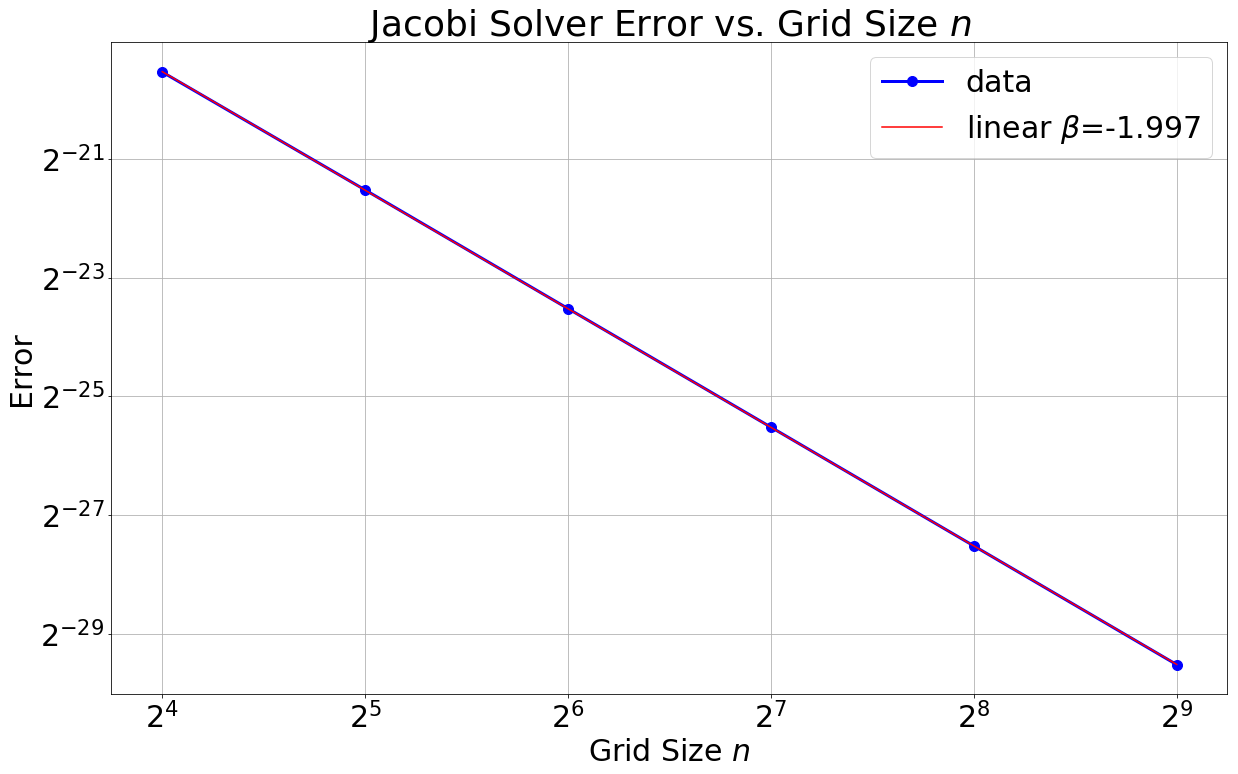
\includegraphics[width=0.90\textwidth]{jacobi_error.png}
\captionof*{figure}{Jacob Error vs. Grid Size}
\end{figure}
\end{center}

      \item How does the runtime scale with the resolution? You can get a rough estimate by using the bash command \texttt{time} when executing your program, like:
    \vspace{3mm}\\ \texttt{./jacobi\_solver.cu n} \vspace{3mm}\\ and using the result for \texttt{real}. \\
Intuitively we would expect that the run-time should scale quadratically with the grid size.
This result is borne out over the range of $n$ tested above.  
The numerical estimate of the slope of $\log(t)$ vs. $\log(n)$ was 1.922.
Here is the plot:
\begin{center}
\begin{figure}
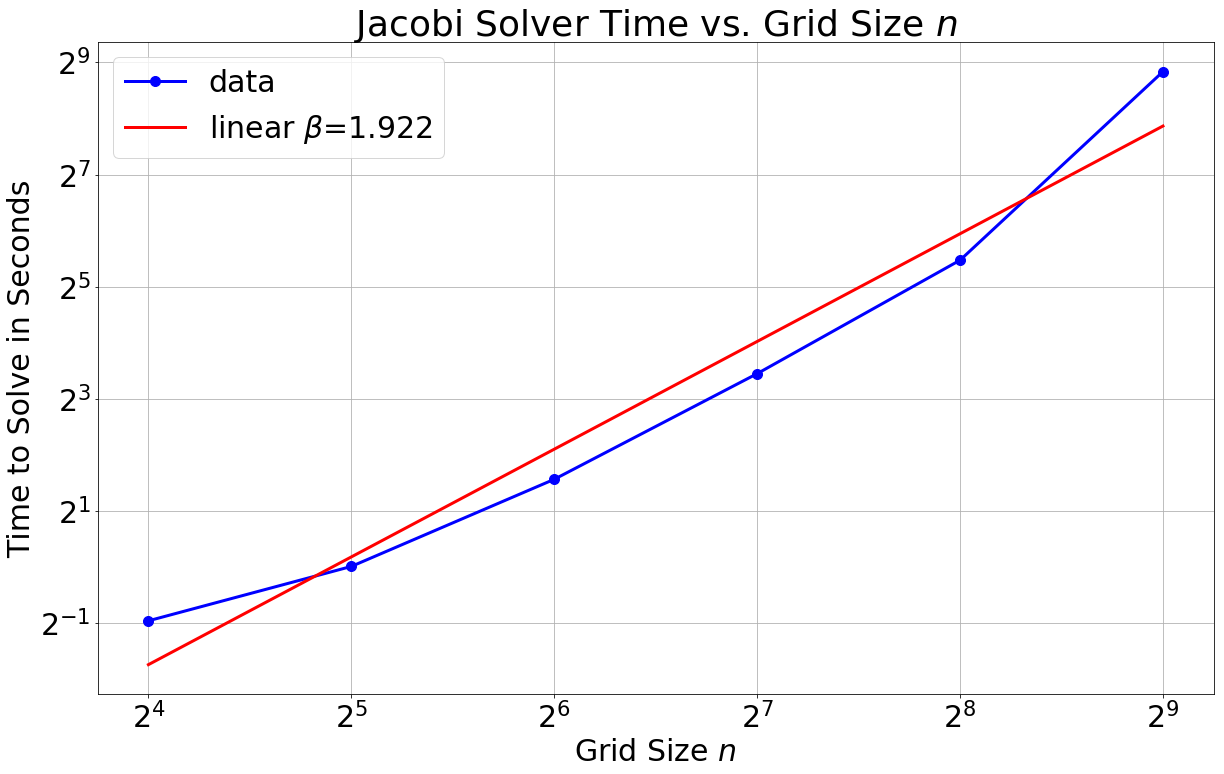
\includegraphics[width=0.90\textwidth]{jacobi_time.png}
\captionof*{figure}{Jacob Runtime vs. Grid Size}
\end{figure}
\end{center}


      \item How does the runtime change as you change the kernel execution configuration?
        e.g., play around the \texttt{MAX\_THREADS\_DIM} parameter as well as different schemes for setting up the thread blocks.
We tried the following choices for the number of threads: 8, 16, 32, 64.
64 threads didn't run; the program terminated immediately.
Run-time with 8, 16, and 32 was 39.940, 44,363, and 36.698 seconds, respectively.
This didn't make a huge amount of sense, because it wasn't even monotonic.
A second trial with n=16 took 40.542 seconds.
If we had to guess, there is probably an advantage to using as many threads as possible
(probably 32 on the Titan-V card), but this advantage likely matters more for larger calculations
than this one for n=256.
      \item Use shared memory in the Jacobi kernel
    \end{itemize}

\end{document}

